\documentclass[]{book}
\usepackage{lmodern}
\usepackage{amssymb,amsmath}
\usepackage{ifxetex,ifluatex}
\usepackage{fixltx2e} % provides \textsubscript
\ifnum 0\ifxetex 1\fi\ifluatex 1\fi=0 % if pdftex
  \usepackage[T1]{fontenc}
  \usepackage[utf8]{inputenc}
\else % if luatex or xelatex
  \ifxetex
    \usepackage{mathspec}
  \else
    \usepackage{fontspec}
  \fi
  \defaultfontfeatures{Ligatures=TeX,Scale=MatchLowercase}
\fi
% use upquote if available, for straight quotes in verbatim environments
\IfFileExists{upquote.sty}{\usepackage{upquote}}{}
% use microtype if available
\IfFileExists{microtype.sty}{%
\usepackage{microtype}
\UseMicrotypeSet[protrusion]{basicmath} % disable protrusion for tt fonts
}{}
\usepackage{hyperref}
\hypersetup{unicode=true,
            pdftitle={STAT 245 Course Notes},
            pdfauthor={Stacy DeRuiter, Calvin University},
            pdfborder={0 0 0},
            breaklinks=true}
\urlstyle{same}  % don't use monospace font for urls
\usepackage{natbib}
\bibliographystyle{apalike}
\usepackage{color}
\usepackage{fancyvrb}
\newcommand{\VerbBar}{|}
\newcommand{\VERB}{\Verb[commandchars=\\\{\}]}
\DefineVerbatimEnvironment{Highlighting}{Verbatim}{commandchars=\\\{\}}
% Add ',fontsize=\small' for more characters per line
\usepackage{framed}
\definecolor{shadecolor}{RGB}{248,248,248}
\newenvironment{Shaded}{\begin{snugshade}}{\end{snugshade}}
\newcommand{\AlertTok}[1]{\textcolor[rgb]{0.94,0.16,0.16}{#1}}
\newcommand{\AnnotationTok}[1]{\textcolor[rgb]{0.56,0.35,0.01}{\textbf{\textit{#1}}}}
\newcommand{\AttributeTok}[1]{\textcolor[rgb]{0.77,0.63,0.00}{#1}}
\newcommand{\BaseNTok}[1]{\textcolor[rgb]{0.00,0.00,0.81}{#1}}
\newcommand{\BuiltInTok}[1]{#1}
\newcommand{\CharTok}[1]{\textcolor[rgb]{0.31,0.60,0.02}{#1}}
\newcommand{\CommentTok}[1]{\textcolor[rgb]{0.56,0.35,0.01}{\textit{#1}}}
\newcommand{\CommentVarTok}[1]{\textcolor[rgb]{0.56,0.35,0.01}{\textbf{\textit{#1}}}}
\newcommand{\ConstantTok}[1]{\textcolor[rgb]{0.00,0.00,0.00}{#1}}
\newcommand{\ControlFlowTok}[1]{\textcolor[rgb]{0.13,0.29,0.53}{\textbf{#1}}}
\newcommand{\DataTypeTok}[1]{\textcolor[rgb]{0.13,0.29,0.53}{#1}}
\newcommand{\DecValTok}[1]{\textcolor[rgb]{0.00,0.00,0.81}{#1}}
\newcommand{\DocumentationTok}[1]{\textcolor[rgb]{0.56,0.35,0.01}{\textbf{\textit{#1}}}}
\newcommand{\ErrorTok}[1]{\textcolor[rgb]{0.64,0.00,0.00}{\textbf{#1}}}
\newcommand{\ExtensionTok}[1]{#1}
\newcommand{\FloatTok}[1]{\textcolor[rgb]{0.00,0.00,0.81}{#1}}
\newcommand{\FunctionTok}[1]{\textcolor[rgb]{0.00,0.00,0.00}{#1}}
\newcommand{\ImportTok}[1]{#1}
\newcommand{\InformationTok}[1]{\textcolor[rgb]{0.56,0.35,0.01}{\textbf{\textit{#1}}}}
\newcommand{\KeywordTok}[1]{\textcolor[rgb]{0.13,0.29,0.53}{\textbf{#1}}}
\newcommand{\NormalTok}[1]{#1}
\newcommand{\OperatorTok}[1]{\textcolor[rgb]{0.81,0.36,0.00}{\textbf{#1}}}
\newcommand{\OtherTok}[1]{\textcolor[rgb]{0.56,0.35,0.01}{#1}}
\newcommand{\PreprocessorTok}[1]{\textcolor[rgb]{0.56,0.35,0.01}{\textit{#1}}}
\newcommand{\RegionMarkerTok}[1]{#1}
\newcommand{\SpecialCharTok}[1]{\textcolor[rgb]{0.00,0.00,0.00}{#1}}
\newcommand{\SpecialStringTok}[1]{\textcolor[rgb]{0.31,0.60,0.02}{#1}}
\newcommand{\StringTok}[1]{\textcolor[rgb]{0.31,0.60,0.02}{#1}}
\newcommand{\VariableTok}[1]{\textcolor[rgb]{0.00,0.00,0.00}{#1}}
\newcommand{\VerbatimStringTok}[1]{\textcolor[rgb]{0.31,0.60,0.02}{#1}}
\newcommand{\WarningTok}[1]{\textcolor[rgb]{0.56,0.35,0.01}{\textbf{\textit{#1}}}}
\usepackage{longtable,booktabs}
\usepackage{graphicx,grffile}
\makeatletter
\def\maxwidth{\ifdim\Gin@nat@width>\linewidth\linewidth\else\Gin@nat@width\fi}
\def\maxheight{\ifdim\Gin@nat@height>\textheight\textheight\else\Gin@nat@height\fi}
\makeatother
% Scale images if necessary, so that they will not overflow the page
% margins by default, and it is still possible to overwrite the defaults
% using explicit options in \includegraphics[width, height, ...]{}
\setkeys{Gin}{width=\maxwidth,height=\maxheight,keepaspectratio}
\IfFileExists{parskip.sty}{%
\usepackage{parskip}
}{% else
\setlength{\parindent}{0pt}
\setlength{\parskip}{6pt plus 2pt minus 1pt}
}
\setlength{\emergencystretch}{3em}  % prevent overfull lines
\providecommand{\tightlist}{%
  \setlength{\itemsep}{0pt}\setlength{\parskip}{0pt}}
\setcounter{secnumdepth}{5}
% Redefines (sub)paragraphs to behave more like sections
\ifx\paragraph\undefined\else
\let\oldparagraph\paragraph
\renewcommand{\paragraph}[1]{\oldparagraph{#1}\mbox{}}
\fi
\ifx\subparagraph\undefined\else
\let\oldsubparagraph\subparagraph
\renewcommand{\subparagraph}[1]{\oldsubparagraph{#1}\mbox{}}
\fi

%%% Use protect on footnotes to avoid problems with footnotes in titles
\let\rmarkdownfootnote\footnote%
\def\footnote{\protect\rmarkdownfootnote}

%%% Change title format to be more compact
\usepackage{titling}

% Create subtitle command for use in maketitle
\providecommand{\subtitle}[1]{
  \posttitle{
    \begin{center}\large#1\end{center}
    }
}

\setlength{\droptitle}{-2em}

  \title{STAT 245 Course Notes}
    \pretitle{\vspace{\droptitle}\centering\huge}
  \posttitle{\par}
    \author{Stacy DeRuiter, Calvin University}
    \preauthor{\centering\large\emph}
  \postauthor{\par}
      \predate{\centering\large\emph}
  \postdate{\par}
    \date{2019-09-09}

\usepackage{booktabs}
\usepackage{amsthm}
\makeatletter
\def\thm@space@setup{%
  \thm@preskip=8pt plus 2pt minus 4pt
  \thm@postskip=\thm@preskip
}
\makeatother

\begin{document}
\maketitle

{
\setcounter{tocdepth}{1}
\tableofcontents
}
\hypertarget{description}{%
\chapter{Description}\label{description}}

This is a set of course notes distributed in STAT 245 at Calvin University in Fall 2019. Contact sld33 at calvin.edu with comments, corrections or suggestions.

\hypertarget{linear-regression}{%
\chapter{Linear Regression}\label{linear-regression}}

You probably learned something about linear regression in a previous course. Here, we briefly review the main concepts of simple linear regression and quickly expand our tool box to multiple regression (with both quantitative and categorical predictors).

\hypertarget{data}{%
\section{Data}\label{data}}

We will consider a small dataset from an article by J.S. Martin and colleagues, titled \href{https://royalsocietypublishing.org/doi/suppl/10.1098/rsbl.2019.0232}{\emph{Facial width-to-height ratio is associated with agonistic and affiliative dominance in bonobos (\textbf{Pan paniscus})}}

Notes: variable \texttt{fWHR} is the facial width-height ratio and \texttt{AssR} is the Assertiveness score of affiliative dominance. \texttt{normDS} is another dominance score. A few figures of the data are below - we will do some more exploration together.

\begin{verbatim}
## Observations: 117
## Variables: 8
## $ Name   <fct> Zuani, Zuani, Zorba, Zorba, Zorba, Zomi, Zomi, Zamba, Z...
## $ Group  <fct> Apenheul, Apenheul, Wilhelma, Wilhelma, Wilhelma, Frank...
## $ Sex    <fct> Female, Female, Male, Male, Male, Female, Female, Male,...
## $ Age    <int> 22, 22, 34, 34, 34, 15, 15, 14, 14, 14, 18, 18, 18, 18,...
## $ fWHR   <dbl> 1.475052, 1.321814, 1.581446, 1.479237, 1.390086, 1.340...
## $ AssR   <dbl> 5.36, 5.36, 2.36, 2.36, 2.36, 3.92, 3.92, 4.74, 4.74, 4...
## $ normDS <dbl> 1.430, 1.430, 2.341, 2.341, 2.341, 3.087, 3.087, 3.035,...
## $ weight <dbl> 24.0, 24.0, NA, NA, NA, NA, NA, 41.6, 41.6, 41.6, 38.0,...
\end{verbatim}

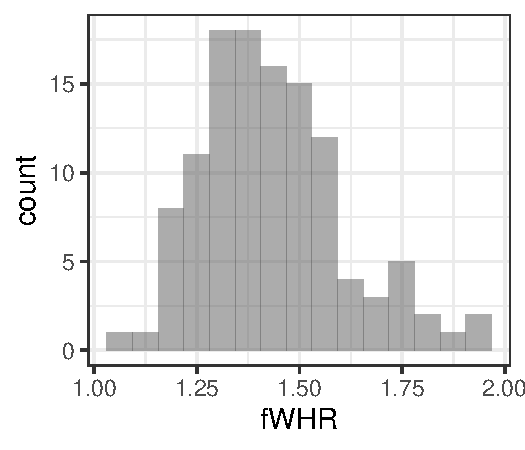
\includegraphics{bookdown-demo_files/figure-latex/view-data-1.pdf} 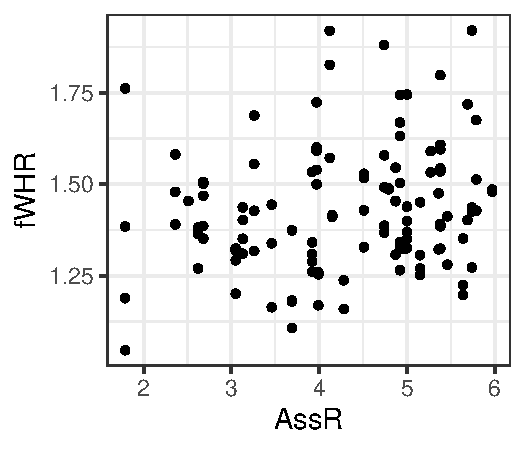
\includegraphics{bookdown-demo_files/figure-latex/view-data-2.pdf}

\hypertarget{simple-linear-regression-residuals-least-squares}{%
\section{Simple linear regression, Residuals \& Least squares}\label{simple-linear-regression-residuals-least-squares}}

First, let's review and consider a simple (one-predictor) linear regression model. Fit the model

\begin{Shaded}
\begin{Highlighting}[]
\NormalTok{slr <-}\StringTok{ }\KeywordTok{lm}\NormalTok{(fWHR }\OperatorTok{~}\StringTok{ }\NormalTok{AssR, }\DataTypeTok{data=}\NormalTok{bonobos)}
\end{Highlighting}
\end{Shaded}

Extract the slope and intercept values:

\begin{Shaded}
\begin{Highlighting}[]
\KeywordTok{coef}\NormalTok{(slr)}
\end{Highlighting}
\end{Shaded}

\begin{verbatim}
## (Intercept)        AssR 
##  1.30685287  0.02918242
\end{verbatim}

Add the regression line to the plot:

\begin{Shaded}
\begin{Highlighting}[]
\KeywordTok{gf_point}\NormalTok{(fWHR }\OperatorTok{~}\StringTok{ }\NormalTok{AssR, }\DataTypeTok{data=}\NormalTok{bonobos) }\OperatorTok\StringTok{ }
\StringTok{  }\KeywordTok{gf_lm}\NormalTok{()}
\end{Highlighting}
\end{Shaded}

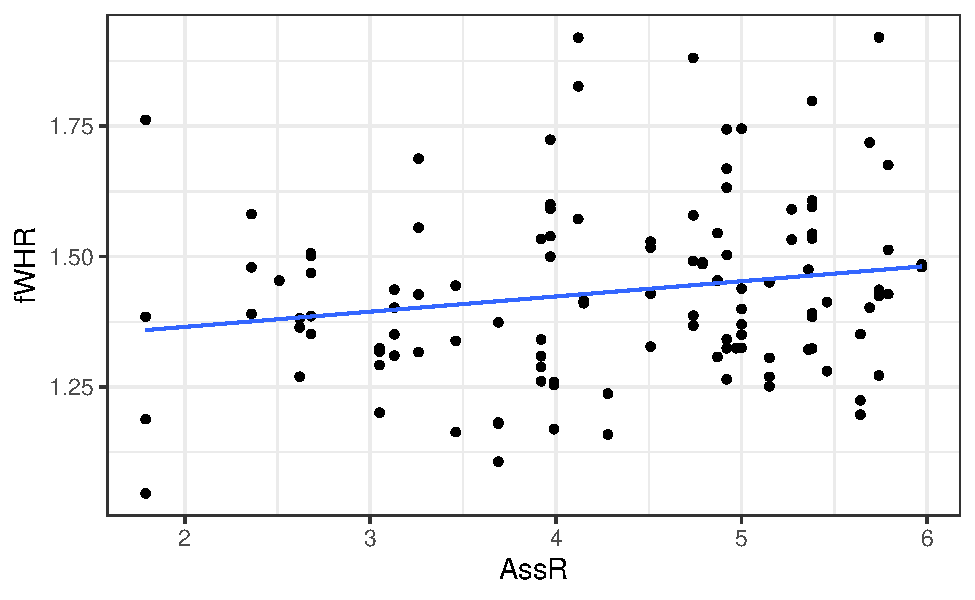
\includegraphics{bookdown-demo_files/figure-latex/lm-scatter-with-line-1.pdf}

\begin{Shaded}
\begin{Highlighting}[]
\KeywordTok{summary}\NormalTok{(slr)}
\end{Highlighting}
\end{Shaded}

\begin{verbatim}
## 
## Call:
## lm(formula = fWHR ~ AssR, data = bonobos)
## 
## Residuals:
##      Min       1Q   Median       3Q      Max 
## -0.31320 -0.11369 -0.01242  0.09008  0.49241 
## 
## Coefficients:
##             Estimate Std. Error t value Pr(>|t|)    
## (Intercept)  1.30685    0.06283  20.801   <2e-16 ***
## AssR         0.02918    0.01420   2.055   0.0421 *  
## ---
## Signif. codes:  0 '***' 0.001 '**' 0.01 '*' 0.05 '.' 0.1 ' ' 1
## 
## Residual standard error: 0.1689 on 115 degrees of freedom
## Multiple R-squared:  0.03542,    Adjusted R-squared:  0.02704 
## F-statistic: 4.223 on 1 and 115 DF,  p-value: 0.04213
\end{verbatim}

\hypertarget{using-lm-to-fit-a-linear-regression-in-r}{%
\subsection{\texorpdfstring{Using \texttt{lm()} to fit a linear regression in R}{Using lm() to fit a linear regression in R}}\label{using-lm-to-fit-a-linear-regression-in-r}}

\vspace{1.5in}

\hypertarget{equation-of-the-fitted-regression-line}{%
\subsection{Equation of the fitted regression line}\label{equation-of-the-fitted-regression-line}}

\vspace{1.5in}

\hypertarget{multiple-regression}{%
\section{Multiple regression}\label{multiple-regression}}

Rarely does our response variable \textbf{really} depend on only one predictor. Can we improve the model by adding more predictors?

\begin{Shaded}
\begin{Highlighting}[]
\NormalTok{mlr <-}\StringTok{ }\KeywordTok{lm}\NormalTok{(fWHR }\OperatorTok{~}\StringTok{ }\NormalTok{AssR }\OperatorTok{+}\StringTok{ }\NormalTok{weight, }\DataTypeTok{data=}\NormalTok{bonobos)}
\KeywordTok{coef}\NormalTok{(mlr)}
\end{Highlighting}
\end{Shaded}

\begin{verbatim}
## (Intercept)        AssR      weight 
## 0.944790930 0.039888045 0.008644299
\end{verbatim}

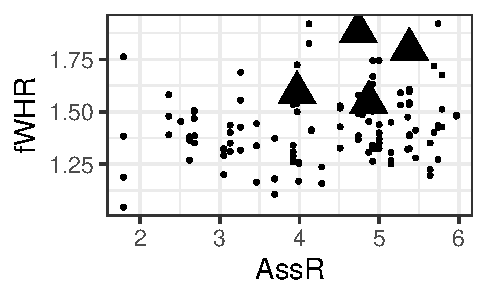
\includegraphics{bookdown-demo_files/figure-latex/mult-reg-plots-1.pdf} 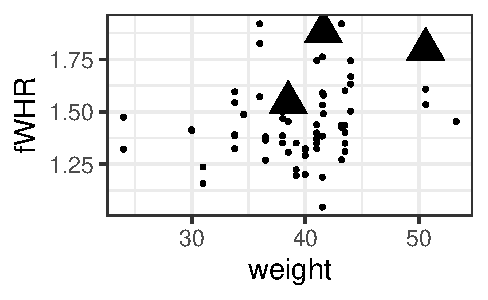
\includegraphics{bookdown-demo_files/figure-latex/mult-reg-plots-2.pdf}

\hypertarget{is-it-really-better}{%
\subsection{Is it really better?}\label{is-it-really-better}}

How do we know if the model with more predictors is ``better''? (For a more detailed answer, wait about a week\ldots{}) But before we can define a ``beter'' model: how did R find the ``best'' intercept and slopes?

\hypertarget{regression-residuals-errors}{%
\subsection{Regression residuals = ``errors''}\label{regression-residuals-errors}}

\vspace{1.25in}

\hypertarget{computing-predictions}{%
\subsection{Computing Predictions}\label{computing-predictions}}

Use the regression equation to compute \textbf{predicted values} for the three data points below:

\begin{verbatim}
##        fWHR AssR weight
## 8  1.880866 4.74   41.6
## 25 1.798387 5.38   50.6
## 41 1.591440 3.97     NA
## 65 1.545019 4.87   38.5
\end{verbatim}

\vspace{2in}

\hypertarget{predictors-with-two-categories}{%
\section{Predictors with two categories}\label{predictors-with-two-categories}}

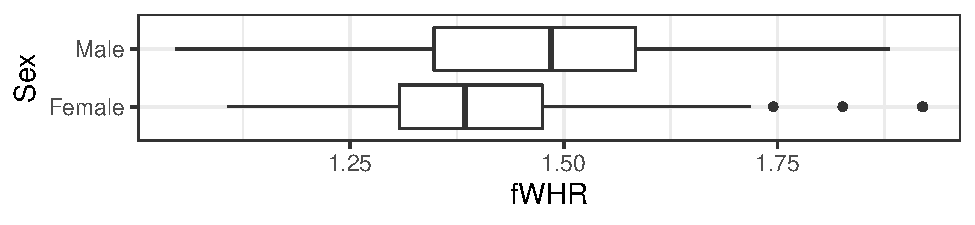
\includegraphics{bookdown-demo_files/figure-latex/unnamed-chunk-2-1.pdf}

\begin{Shaded}
\begin{Highlighting}[]
\NormalTok{mlr2 <-}\StringTok{ }\KeywordTok{lm}\NormalTok{(fWHR }\OperatorTok{~}\StringTok{ }\NormalTok{AssR }\OperatorTok{+}\StringTok{ }\NormalTok{weight }\OperatorTok{+}\StringTok{ }\NormalTok{Sex, }\DataTypeTok{data =}\NormalTok{ bonobos)}
\KeywordTok{coef}\NormalTok{(mlr2)}
\end{Highlighting}
\end{Shaded}

\begin{verbatim}
## (Intercept)        AssR      weight     SexMale 
## 1.065420976 0.058435841 0.002257142 0.128484275
\end{verbatim}

How does the model incorporate this covariate mathematically?

\vspace{1.75in}

\hypertarget{predictors-with-more-categories}{%
\subsection{Predictors with more categories}\label{predictors-with-more-categories}}

\begin{Shaded}
\begin{Highlighting}[]
\KeywordTok{gf_boxplot}\NormalTok{(fWHR }\OperatorTok{~}\StringTok{ }\NormalTok{Group, }\DataTypeTok{data =}\NormalTok{ bonobos)}
\end{Highlighting}
\end{Shaded}

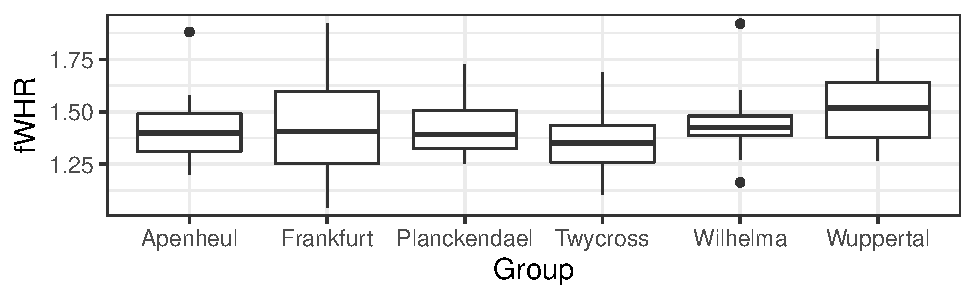
\includegraphics{bookdown-demo_files/figure-latex/unnamed-chunk-4-1.pdf}

\begin{Shaded}
\begin{Highlighting}[]
\NormalTok{mlr3 <-}\StringTok{ }\KeywordTok{lm}\NormalTok{(fWHR }\OperatorTok{~}\StringTok{ }\NormalTok{AssR }\OperatorTok{+}\StringTok{ }\NormalTok{weight }\OperatorTok{+}\StringTok{ }\NormalTok{Sex }\OperatorTok{+}\StringTok{ }\NormalTok{Group, }\DataTypeTok{data =}\NormalTok{ bonobos)}
\KeywordTok{coef}\NormalTok{(mlr3)}
\end{Highlighting}
\end{Shaded}

\begin{verbatim}
##       (Intercept)              AssR            weight           SexMale 
##       1.007734691       0.064361973       0.003458979       0.124854271 
##    GroupFrankfurt GroupPlanckendael     GroupTwycross     GroupWilhelma 
##       0.037426358      -0.008464572      -0.112907589       0.011186724 
##    GroupWuppertal 
##      -0.004364826
\end{verbatim}

How does the model incorporate \textbf{this} covariate mathematically?

\vspace{1.75in}

\hypertarget{literature}{%
\chapter{Literature}\label{literature}}

Here is a review of existing methods.

\hypertarget{methods}{%
\chapter{Methods}\label{methods}}

We describe our methods in this chapter.

\hypertarget{applications}{%
\chapter{Applications}\label{applications}}

Some \emph{significant} applications are demonstrated in this chapter.

\hypertarget{example-one}{%
\section{Example one}\label{example-one}}

\hypertarget{example-two}{%
\section{Example two}\label{example-two}}

\hypertarget{final-words}{%
\chapter{Final Words}\label{final-words}}

We have finished a nice book.

\hypertarget{intro}{%
\chapter{Introduction}\label{intro}}

You can label chapter and section titles using \texttt{\{\#label\}} after them, e.g., we can reference Chapter \ref{intro}. If you do not manually label them, there will be automatic labels anyway, e.g., Chapter \ref{methods}.

Figures and tables with captions will be placed in \texttt{figure} and \texttt{table} environments, respectively.

\begin{Shaded}
\begin{Highlighting}[]
\KeywordTok{par}\NormalTok{(}\DataTypeTok{mar =} \KeywordTok{c}\NormalTok{(}\DecValTok{4}\NormalTok{, }\DecValTok{4}\NormalTok{, }\FloatTok{.1}\NormalTok{, }\FloatTok{.1}\NormalTok{))}
\KeywordTok{plot}\NormalTok{(pressure, }\DataTypeTok{type =} \StringTok{'b'}\NormalTok{, }\DataTypeTok{pch =} \DecValTok{19}\NormalTok{)}
\end{Highlighting}
\end{Shaded}

\begin{figure}

{\centering 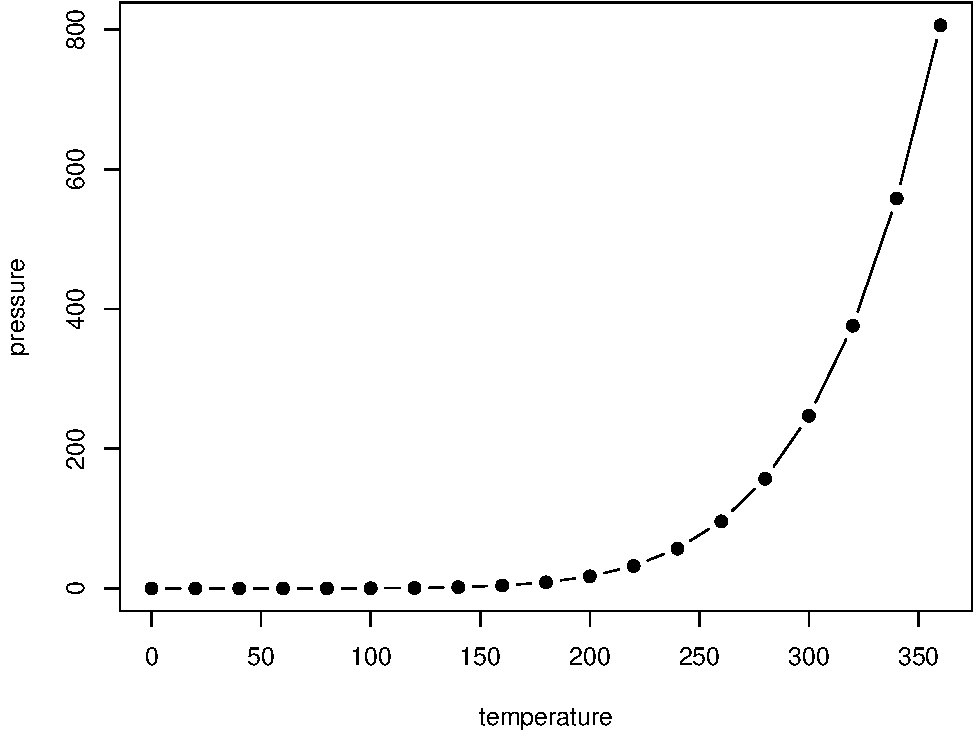
\includegraphics[width=0.8\linewidth]{bookdown-demo_files/figure-latex/nice-fig-1} 

}

\caption{Here is a nice figure!}\label{fig:nice-fig}
\end{figure}

Reference a figure by its code chunk label with the \texttt{fig:} prefix, e.g., see Figure \ref{fig:nice-fig}. Similarly, you can reference tables generated from \texttt{knitr::kable()}, e.g., see Table \ref{tab:nice-tab}.

\begin{Shaded}
\begin{Highlighting}[]
\NormalTok{knitr}\OperatorTok{::}\KeywordTok{kable}\NormalTok{(}
  \KeywordTok{head}\NormalTok{(iris, }\DecValTok{20}\NormalTok{), }\DataTypeTok{caption =} \StringTok{'Here is a nice table!'}\NormalTok{,}
  \DataTypeTok{booktabs =} \OtherTok{TRUE}
\NormalTok{)}
\end{Highlighting}
\end{Shaded}

\begin{table}[t]

\caption{\label{tab:nice-tab}Here is a nice table!}
\centering
\begin{tabular}{rrrrl}
\toprule
Sepal.Length & Sepal.Width & Petal.Length & Petal.Width & Species\\
\midrule
5.1 & 3.5 & 1.4 & 0.2 & setosa\\
4.9 & 3.0 & 1.4 & 0.2 & setosa\\
4.7 & 3.2 & 1.3 & 0.2 & setosa\\
4.6 & 3.1 & 1.5 & 0.2 & setosa\\
5.0 & 3.6 & 1.4 & 0.2 & setosa\\
\addlinespace
5.4 & 3.9 & 1.7 & 0.4 & setosa\\
4.6 & 3.4 & 1.4 & 0.3 & setosa\\
5.0 & 3.4 & 1.5 & 0.2 & setosa\\
4.4 & 2.9 & 1.4 & 0.2 & setosa\\
4.9 & 3.1 & 1.5 & 0.1 & setosa\\
\addlinespace
5.4 & 3.7 & 1.5 & 0.2 & setosa\\
4.8 & 3.4 & 1.6 & 0.2 & setosa\\
4.8 & 3.0 & 1.4 & 0.1 & setosa\\
4.3 & 3.0 & 1.1 & 0.1 & setosa\\
5.8 & 4.0 & 1.2 & 0.2 & setosa\\
\addlinespace
5.7 & 4.4 & 1.5 & 0.4 & setosa\\
5.4 & 3.9 & 1.3 & 0.4 & setosa\\
5.1 & 3.5 & 1.4 & 0.3 & setosa\\
5.7 & 3.8 & 1.7 & 0.3 & setosa\\
5.1 & 3.8 & 1.5 & 0.3 & setosa\\
\bottomrule
\end{tabular}
\end{table}

You can write citations, too. For example, we are using the \textbf{bookdown} package \citep{R-bookdown} in this sample book, which was built on top of R Markdown and \textbf{knitr} \citep{xie2015}.

\bibliography{book.bib,packages.bib}


\end{document}
